\documentclass[12pt,a4paper]{article}
\usepackage{natbib}         % Pour la bibliographie
\usepackage{url}            % Pour citer les adresses web
\usepackage[T1]{fontenc}    % Encodage des accents
\usepackage[utf8]{inputenc} % Lui aussi
\usepackage[french]{babel} % Pour la traduction française
\usepackage{numprint}       % Histoire que les chiffres soient bien

\usepackage{amsmath}        % La base pour les maths
\usepackage{mathrsfs}       % Quelques symboles supplémentaires
\usepackage{stmaryrd}
\usepackage{amssymb}        % encore des symboles.
\usepackage{amsfonts}       % Des fontes, eg pour \mathbb.
\usepackage{blindtext}
\usepackage{algorithm, algpseudocode}
\usepackage{tikz, tkz-graph}
\usepackage{multicol}
\usepackage{caption, subcaption}
\usepackage[left=2cm, right=2cm, top=2cm, bottom=2cm]{geometry}
\usepackage{float}

\usepackage[svgnames]{xcolor} % De la couleur
\usepackage{geometry}       % Gérer correctement la taille

%%% Si jamais vous voulez changer de police: décommentez les trois 
%\usepackage{tgpagella}
%\usepackage{tgadventor}
%\usepackage{inconsolata}


\usepackage{graphicx} % inclusion des graphiques
\usepackage{wrapfig}  % Dessins dans le texte.

\usepackage{tikz}     % Un package pour les dessins (utilisé pour l'environnement {code})


% Mettez votre titre et votre nom ci-après
\title{Rapport de TIPE \\
Implémenter un réseau pair à pair à l'aide de b-couplages stables}
\author{S Roux, MPI, \oldstylenums{2025}-\oldstylenums{2026}}
%% À décommenter si vous ne voulez pas que la date apparaisse explicitement
%\date{}


% NB: le script TeXcount permet de compter les mots utilisés dans chaque section d'un document LaTeX. Vous en trouverez une version en ligne à l'adresse
% http://app.uio.no/ifi/texcount/online.php
% Il suffit d'y copier l'ensemble du présent document (via Ctrl-A/Ctrl-C puis Ctrl-V dans la fenêtre idoine) pour obtenir le récapitulatif tout en bas de la page qui s'ouvre alors.

% Pour récupérer les bonnes entrées bibliographiques, je vous conseille l'usage de scholar.google.fr pour les recherches
% et la récupération des entrée BibTeX comme décrit dans cette vidéo: https://www.youtube.com/watch?v=X-9T2Oaj-5A

% Quelques macros utiles
% La dérivée temporelle, tellement courante en physique, avec les d droits
\newcommand{\ddt}[1]{\frac{\dd #1}{\dd t}}
% Des parenthèses, crochets et accolades qui s'adaptent automatiquement à la taille de ce qu'il y a dedans
\newcommand{\pa}[1]{\left(#1\right)}
\newcommand{\pac}[1]{\left[#1\right]}
\newcommand{\paa}[1]{\left\{#1\right\}}
% Un raccourci pour écrire une constante
\newcommand{\cte}{\text{C}^{\text{te}}}
% Pour faire des indices en mode texte (comme les énergie potentielles)
\newcommand{\e}[1]{_{\text{#1}}}
% Le produit vectoriel a un nom bizarre:
\newcommand{\vectoriel}{\wedge}

\begin{document}

\maketitle

\tableofcontents

\section{Introduction}


Les réseaux pair à pair permettent le partage de fichiers de manière décentralisée, où chaque utilisateur se comporte comme un serveur, capable de partager les fichiers qu'il possède [1]. Chaque utilisateur ne peut partager et recevoir qu'un nombre limité de fichiers à la fois, ce qui mène à prioriser certains transferts plutôt que d'autres. Une problématique émerge donc: comment optimiser, à chaque instant, le transfert des segments du fichier (origine et destination), tout en garantissant un temps de convergence algorithmique suffisamment faible (soit inférieur au temps caractéristique d’évolution du réseau)? 


Un \textit{réseau} désignera par la suite un ensemble $R$ d'utilisateurs, nommés $noeuds$. Pour chaque noeuds $(n, p)\in R^2$, $\sigma(n, p)$ désigne un nombre positif nommé la \textit{marque de p selon n}. La liste $Pref(n)$, nommée \textit{liste de préférence}, ordonne l'ensemble des autres noeuds du réseau par marque croissante. $R$ est dit \textit{statique} s'il est constant au cours du temps, et au contraire \textit{dynamique} si des noeuds peuvent y être ajoutés et retirés.
On nomme \textit{graphe de préférence de $R$} le graphe orienté dont les sommets sont les noeuds de $R$ et où une unique arête pointe de chaque noeud $n$ vers le noeud $p$ de marque maximale: 
\begin{equation}
\sigma(n, p)=\max\limits_{q} \sigma(n, q)
\end{equation}

Notons que chaque noeud y est de degré sortant 1. On dira qu'un graphe de préférence est cyclique s'il contient un cycle de longeur au moins 3.

\vspace{0.2cm}
\begin{figure}[H]
  \centering
  \begin{tikzpicture}
  \centering
        \SetUpEdge[lw = 1.5pt,
        color = orange,
        labelcolor = white]
        \GraphInit[vstyle=Normal] \SetGraphUnit{3}
        \tikzset{VertexStyle/.append style={fill = red!50}}
        \Vertex{B}
        \EA(B){A} \NO(B){C} \EA(C){D}
        \EA(D){E} \SO(E){F}
        \tikzset{EdgeStyle/.style={->}}
        \Edge(B)(C)
        \Edge(C)(D)
        \Edge(D)(E)
        \Edge(E)(F)
        \Edge(A)(D)
        \tikzset{EdgeStyle/.style={bend left, ->}}
        \Edge(F)(E)
  \end{tikzpicture}
  \caption{Graphe de préférence \textit{acyclique} associé à un réseau \{A, B, C, D, E, F, G\}}
\end{figure}

\vspace{0.2cm}


Pour $b\in \mathbb{N}^*$, un \textit{$b$-couplage} sur un réseau $R$ désigne une partie $C\in$ R² telle que 
\begin{equation}
\forall n\in N, \space \sharp\{\{n, p\}\space  | \space p \in N\} \space \leq \space b
\end{equation}


Ce b-couplage $C$ est dit \textit{stable} s'il est de cardinal maximal et si 
\begin{equation}
\forall \{n, p\}\in C, \ \forall \{n', p'\} \in N^{2},\  \sigma(n, p) > \sigma(n, p') \ ou \ \sigma(p, n) > \sigma(p, n')
\end{equation}


En l'absence d'ambiguïté, on appelera $C$ un \textit{couplage}. 


Le choix des transferts de données à effectuer peut être vu comme un problème de couplage stable dans le réseau forméoblème de couplage stable dans le réseau formé par l'ensemble des utilisateurs [2]. La marque $\sigma(n, p)$ y représente l'attractivité de $p$ selon $n$, qui peut par exemple dépendre de la connection de $p$ et des paquets dont $p$ dispose. Intuitivement, un $b$-couplage stable contient pour chaque noeud ses arêtes de plus grande marque, en essayant ainsi de satisfaire un maximum de noeuds. 


On commence par implémenter \(Section 2.1\) un algorithme de calcul de b-couplage dans un réseau statique. 
Deux problématiques théoriques émergent ensuite lors de l'implémentation d'un réseau par des couplages stables. 
Premièrement, il s'agit d'étendre les algorithmes de calcul de b-couplage aux réseaux dynamiques. 
Naïvement, il est possible de recalculer un couplage après toute modification (Section 2.2).
Toutefois le manque de pertinence algorithmique de cette solution (qu'on nommera $DYNA1$) invite à considérer une extension plus réfléchie s'appuyant sur une modification locale du couplage (Section 2.3) qu'on nommera $DYNA2$. 
$DYNA1$ servira néanmoins à quantifier les performances algorithmiques de $DYNA2$. 
Deuxièmement, l'existence d'un $b$-couplage stable n'est pas garantie dans tout réseau; néanmoins, Matthieu (2007) montre qu'un $b$-couplage stable existe systématiquement dans un réseau dont le graphe de préférence est acyclique, ce qui est possible si par exemple la fonction $\sigma$ est symmétrique et injective. 
Certains critères de préférence peuvent toutefois donner naissance à des graphes de préférence cycliques.
La détermination systématique d'un couplage stable étant impossible, on s'intéressera en Section 3 à la possibilité de déterminer une approximation de couplage stable.


\section{Implémentation d'un algorithme de calcul de $b$-couplage stable dans un réseau dynamique}
\subsection{Calcul d'un b-couplage stable dans un réseau statique}


On fixe dans la suite un réseau statique $R$ et un entier $b\in \mathbb{N}^*$. Montrons un théorème annoncé en introduction:

\vspace{0.2cm}
\textbf{Théorème: }  Si $\sigma$ est symétrique et injective, alors le graphe de préférence $G$ de $R$ ne contient pas de cycle de longeur au moins 3.

\vspace{0.2cm}
\textit{Démonstration: } On suppose par l'absurde l'existence d'un cycle $(n_0, n_1, ..., n_p)$ dans $G$. Soit $i\in \llbracket2, n-1\rrbracket$. Par construction, 
\begin{equation}
    \sigma(n_i, n_{i+1}) = \max\limits_{p} \sigma(n_i, p) > \sigma(n_i, n_{i-1}) = \sigma(n_{i-1}, n_i)
\end{equation}
L'inégalité est stricte par injectivité de $\sigma$. On obtient donc que le cycle est strictement croissant selon $\sigma$, ce qui est absurde car alors 
\begin{equation}
    \sigma(n_0, n_1) < ... < \sigma(n_{p}, n_0) < \sigma(n_0, n_1)
\end{equation}
$\square$
\vspace{0.2cm}

En complément de ce résultat, Mathieu (2007) montre qu'un b-couplage stable existe dès lors que $G$ est acyclique. Par soucis de concision, la démonstration n'est pas développée ici. 

A cet effet, ce dernier implémente un algorithme de calcul de $b$-couplage stable inspiré par l'algorithme de Gale et Shapley. On le nommera $STATIQUE(R, b)$. 
On définit une \textit{paire bloquante} comme une paire $\{n, p\}$ de noeuds non couplés telle que, soit $n$ ou $p$ n'est pas complètement couplé, soit $n$ et $p$ préfèrent se coupler ensemble plutôt qu'avec le noeud de pire marque avec lequel chacun est couplé.

\vspace{0.2cm}
  \begin{figure}[H]
    \centering
    \begin{tikzpicture}
        \centering
        \SetUpEdge[lw = 1.5pt,
        color = red,
        labelcolor = white]
        \GraphInit[vstyle=Normal] \SetGraphUnit{3}
        \tikzset{VertexStyle/.append style={fill = red!50}}
        \Vertex{A}
        \NO(A){B} \EA(B){C}
        \tikzset{EdgeStyle/.style={-}}
        \Edge(A)(B)
        \tikzstyle{EdgeStyle}=[dotted, color=black]
        \Edge(A)(C)
        \node[anchor=south] at (B.north) {[A; C]};
        \node[anchor=east] at (A.west) {[C; B]};
        \node[anchor=south] at (C.north) {[A; B]};
    \end{tikzpicture}
    \caption{Réseau \{A, B, C\}. A côté de chaque noeud est représenté une liste de préférence. Une liaison rouge représente un couple dans le 1-couplage. La ligne en pointillés noire représente le couple que préfèreraient former A et C. \{A, C\} est une paire bloquante.}
  \end{figure}
\vspace{0.2cm} 

Par définition, le couplage est stable s'il n'existe pas de paire bloquante. 
$STATIQUE$ consiste à retirer une à une les paires bloquantes.

\begin{algorithm}
  \caption{Calcul b-couplage stable statique}
  \begin{algorithmic}
    \Procedure{Statique}{$r,b$}\Comment{Un réseau non coupl\'e $r$, et $b\in\mathbb{N}^*$}
    \While{$Il\ existe\ une\ paire\ bloquante$}
        \State Soit \{n, p\} une paire bloquante prise aléatoirement
        \State Si\ n\'ecessaire,\ d\'ecoupler\ le\ pire\ partenaire\ de\ $n$\ (resp.\ $p$)
        \State Coupler $n$ et $p$
    \EndWhile
    \EndProcedure
    \end{algorithmic}

\end{algorithm}

D'après ce qui précède, $STATIQUE$ construit bien un couplage stable.

La preuve de terminaison de $STATIQUE$ ainsi que certaines précisions sur les choix d'implémentation sont développés en annexe 4.1.

Les figures  sont obtenues à partir de réseau dont les listes de préférences sont produites par la construction de Erd\H{o}s-Rényi: tout noeud $Y$ a probabilité $p$ d'être présente dans la liste de préférence de $X$. La marque $\sigma(X, Y)$ est alors choisie aléatoirement. 
On note expérimentalement que le temps de convergence ne dépend pas de $p$. 
On se place donc par la suite dans le cas où $p=1$. 

L'exécution de cet algorithme permet de produire la figure 3.(a).
Notons que l'implémentation pratique avait pour objectif d'exposer grossièrement les dépendances de chaque variable et était peu optimisée. 
Par suite, une meilleure complexité serait possible. 


\begin{figure}
\centering
\begin{subfigure}{.5\textwidth}
  \centering
  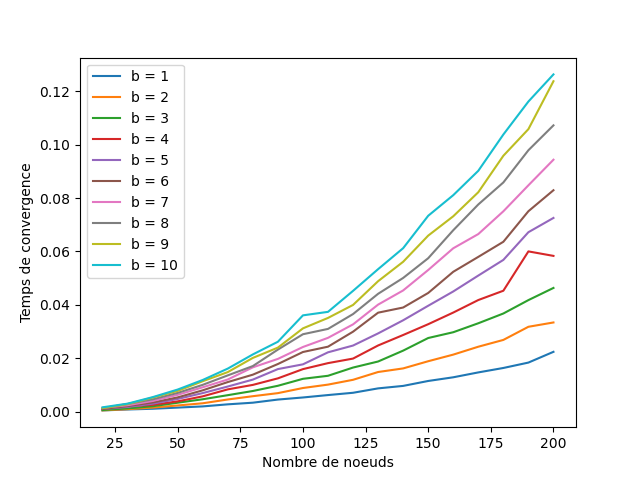
\includegraphics[width=\linewidth]{chart_fab_p=1.png}
  \caption{}
\end{subfigure}%
\begin{subfigure}{.5\textwidth}
  \centering
  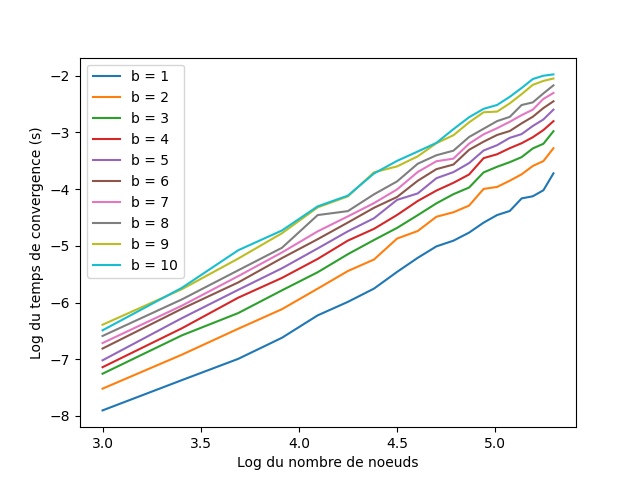
\includegraphics[width=\linewidth]{chart_fab_log.png}
  \caption{}
\end{subfigure}
\caption{Temps de convergence linéaire \(a\) et logarithmique \(b\) de $STATIQUE$}
\end{figure}


D'après l'allure de cette courbe, on s'attend que la complexité de l'algorithme soit de l'ordre de $O(2^{n+b})$, ce qui est mis en évidence par la courbe logarithmique de la figure 3.(b), dont le profil est proche de celui d'une fonction linéaire. 


\subsection{Adaptation dynamique naïve de l'algorithme de calcul}

On s'intéresse ici à une adaptation naïve de l'algorithme précédant, consistant à itérer $STATIQUE$ depuis un réseau de couplage vide à chaque modification du réseau. 
Par correction de $STATIQUE$, on garantit donc la conservation d'un couplage stable après convergence. 
On trace en figure 4.(a) les temps de convergence après ajout successifs de 200 noeuds à partir d'un réseau de 10 noeuds. 
Comme attendu, les profils de temps de convergence sont similaires à ceux obtenus en 3.(a).


\begin{figure}
\centering
\begin{subfigure}{.5\textwidth}
  \centering
  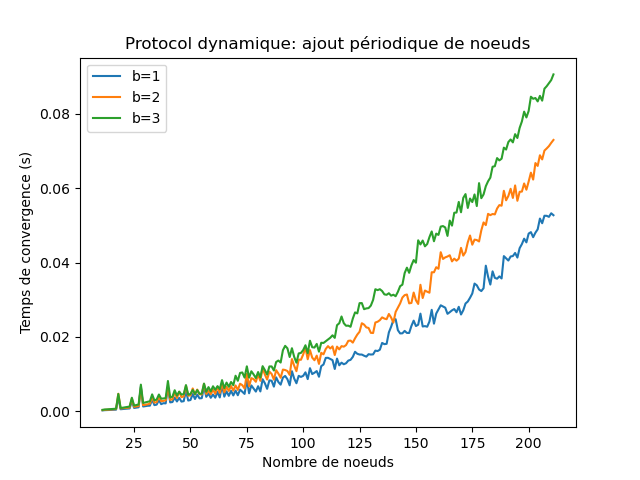
\includegraphics[width=1.1\linewidth]{chart_dyna_t.png}
  \caption{}
\end{subfigure}%
\begin{subfigure}{.5\textwidth}
  \centering
  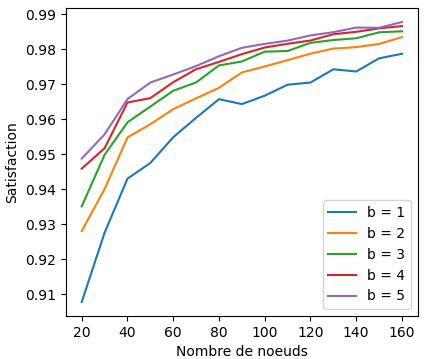
\includegraphics[width=\linewidth]{chart_fab_sat.png}
  \caption{}
\end{subfigure}
\caption{}
\end{figure}


\subsection{Adaptation dynamique de l'algorithme de calcul par modification locale}


Lors de l'ajout d'un noeud $n$, on peut espérer que seuls les noeuds de plus grande marque selon $n$ modifieront leur couplage. 
Idem, lors du retrait d'un noeud $n$, les couplages des noeuds couplés à $n$ seront \textit{a priori} les seuls à être directement modifiés. 
Ainsi, la modification du réseau est une opération locale à la suite de laquelle on peut proposer une modification seulement locale du couplage dans l'optique de "réparer" la perturbation occasionnée.
 J'ai donc implémenté une adaptation de $STATIQUE$ dans laquelle le retrait d'un noeud $n$ entraîne la suppression 
\begin{itemize}
\item des arêtes $\{n, p\}$ dans le couplage, et pour chaque tel $p$,
\item des arêtes $\{q, r\}$ si $\sigma(q, r) < \sigma(q, p)$ ou $\sigma(q, r) < \sigma(r, p)$
\end{itemize}

En effet, les couples $\{q, p\}$ ou $\{r, p\}$ seront des paires bloquantes et nuisent à la stabilité du couplage. On peut continuer ce processus d'élimination de couples en appliquant la deuxième étape à $p=q$ et $p=r$, et ainsi de suite. On garantit de cette manière de retrouver toutes les paires bloquantes du réseau. Enfin, on relance $STATIQUE$ sur le réseau restant pour retrouver un couplage stable. 

Dans le cas d'un ajout d'un noeud $n$, on procède à partir du point listé 2 pour $p=n$.

Le processus de retrait de couple reste coûteux: on parcourt plusieurs fois le couplage et plus il y a de paires bloquantes recensées, plus $STATIQUE$ sera long. Dans une démarche simplificatrice, on ne retire que les couples listés plus haut: on risque alors de manquer des paires bloquantes et de finalement trouver un couplage non stable. Pour mesurer cela, on introduit la \textit{fonction de satisfaction S}:
\begin{equation}
S = \frac{1}{|R|}\sum_{i\in R}{S_i} = \frac{1}{|R|}\sum_{i\in R}{(\frac{c_i}{b}+\sum_{j}{\frac{R_i - C_i}{bL_i}})}
\end{equation}

où, pour $i$ et $j$ deux noeuds, $c_i$ désigne le nombre de couples dans lesquels $i$ intervient, $R_j$ le rang de $j$ dans $Pref(i)$, $C_j$ le rang de $j$ parmi les noeuds couplés avec $i$ et $L_i = |Pref(i)|$.

Intuitivement, plus $S_i$ est proche de 1, plus $i$ est satisfait par son couplage. Moyenner les $S_i$ permet donc de mesurer la satisfaction générale du réseau. La figure 2.(b) permet de confirmer cette intuition: la satisfaction obtenue à l'issue de $STATIQUE$ présente de hauts taux de satisfaction pour $|R| \geq 50$.

Comme montré en figure 3, l'implémentation de cette nouvelle adaptation par modification locale pour le cas d'ajouts successifs de noeuds converge sensiblement plus rapidement que dans le cas naïf. La courbe du temps de convergence s'est affaissée en un profil linéaire. De surcroît, le couplage ainsi déterminé est satisfaisant si $|R| \geq 50$. 

En figure 4, on considère l'adaptation dans le cas d'ajouts et retraits successifs. Au fur et à mesure des ajouts et retraits, chaque liaison est succeptible d'être supprimée. J'ai donc mesuré le nombre de tours (d'ajouts ou de retraits) que dure en moyenne un couple. Cette donnée permet d'évaluer le temps dont dispose chaque couple de noeuds pour opérer leur transfert de données via cette liaisons. Par exemple, pour un réseau réel de 300 utilisateurs connectés, et chaque utilisateur reste connecté en moyenne 10 minutes, un noeud est ajouté/retiré chaque seconde, ce qui est grand devant le temps de convergence de l'algorithme. Du point de vue très simplificateur de ce modèle de réseau, cette méthode de modification locale du couplage semble être adaptée à une utilisation dans le cadre de réseaux pairs à pairs. 


\begin{figure}
  \centering
  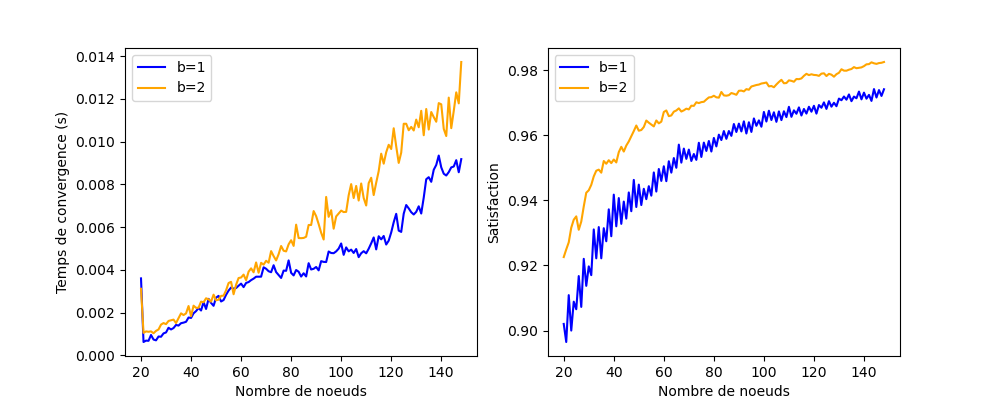
\includegraphics[width=\linewidth]{chart_adap_add.png}
  \caption{}
\end{figure}
\begin{figure}
  \centering
  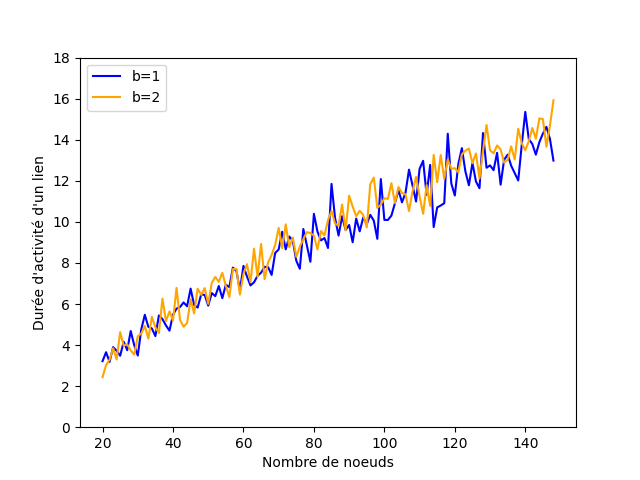
\includegraphics[width=\linewidth]{chart_adap_span.png}
  \caption{}
\end{figure}

\section{S'affranchir de la condition d'acyclicité}

Comme expliqué en introduction, un $b$-couplage stable n'existe pas toujours, notamment si le graphe de préférence est cyclique. 
Dans l'exemple suivant, on représente en rouge un 1-couplage, mais il n'existe pas de couplage stable.

\vspace{0.2cm}
  \begin{figure}[H]
    \centering
    \begin{tikzpicture}
      \centering
        \SetUpEdge[lw = 1.5pt,
        color = red,
        labelcolor = white]
        \GraphInit[vstyle=Normal] \SetGraphUnit{3}
        \tikzset{VertexStyle/.append style={fill = red!50}}
        \Vertex{A}
        \node[anchor=east] at (A.west) {[B; C]};
        \Vertex[x=1.5, y=2]{B}
        \Vertex[x=3, y=0]{C}
        \node[anchor=east] at (B.west) {[C; A]};
        \node[anchor=west] at (C.east) {[A; B]};
        \tikzstyle{EdgeStyle}=[color=red, -]
        \Edge(A)(B)
        \tikzstyle{EdgeStyle}=[color=black, dotted]
        \Edge(B)(C)
        \Edge(C)(A)
    \end{tikzpicture}
    \caption{On reprend le formalisme de la figure 2}
  \end{figure}
\vspace{0.2cm}



J'ai essayé d'adapter $STATIQUE$ au cas de graphes de préférences cycliques en détruisant une arête dès qu'un cycle était détécté, puis un noeud si sa liste de préférence a été complètement vidée. 
Les résultats de convergence en figure 5 sont peu encourageant: non seulement l'algorithme converge plusieurs centaines de fois plus lentement que $STATIQUE$, mais la satisfaction est très basse. 
En l'état, cette adaptation n'a pas d'utilité pratique.


\begin{figure}
  \centering
  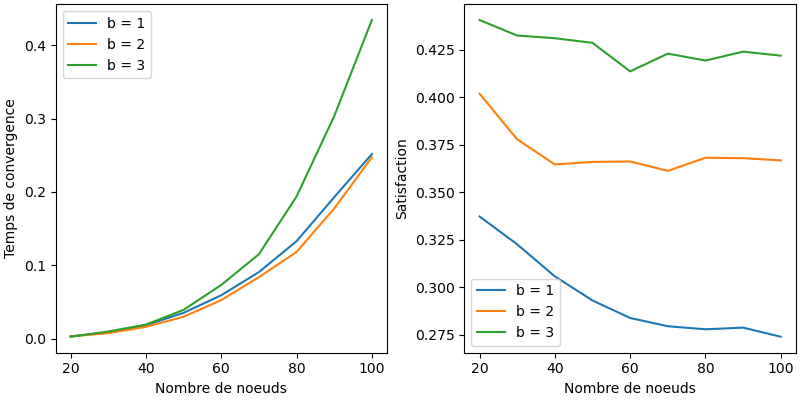
\includegraphics[width=\linewidth]{chart_cyc_t_sat.png}
  \caption{Temps de convergence et satisfaction après $CYCLIQUE$}
\end{figure}

\section{Conclusions et perspectives}



L'implémentation des réseaux pair à pair à la lumière de la théorie des couplages stables est un domaine riche et prometteur, permettant d'optimiser les liaisons faites en fonction de préférences de chaque utilisateur. Cela n'est cependant possible que dans le cas de préférences donnant naissance à un graphe de préférences acyclique, condition dont il n'est pas simple de s'affranchir. 

Dans le cadre de la forte simplification qui est faite ici du protocole de couplage mis en place par les réseaux pair à pair, le couplage par b-couplages stables semble converger suffisamment rapidement pour le partage de segment de données entre les utilisateurs. 
Il serait intéressant d'implémenter un algorithme de couplage couramment utilisé dans les réseaux pair à pair afin de pouvoir comparer sa performance à celle de mon implémentation.

Il ressort de mon étude que la satisfaction semble être une mesure plus adéquate que celle de stabilité pour quantifier la qualité d'un couplage. 
En effet, la stabilité est une notion binaire, peu adaptée à un problème d'optimisation et à la recherche d'un facteur d'approximation. 
La satisfaction étant un nombre entre 0 et 1, elle est pour sa part adaptée à un tel problème. 

De surcroît, l'algorithme d'approximation d'un couplage de satisfaction maximale proposé par G. Georgiadis et F. Papatriantafilou (2007) est fonctionnel dans le cas de graphes de préférences cycliques. 
Dans le cas des couplages stables, il s'agit d'une contrainte de laquelle on ne peut pas s'affranchir simplement: l'adaptation que j'ai proposée a échoué; il serait donc intéressant d'approfondir les raisons de son échec et d'en déduire une nouvelle adaptation plus pertinente.



\section{Annexes}
\subsection{Preuve de terminaison de $STATIQUE$}


La preuve de terminaison de l'algorithme repose sur la notion de \textit{paire aimante}. 
Une paire \{n, p\} est dite aimante si $n$ \textit{et} $p$ sont chacun premier dans la liste de préférence de l'autre. En d'autres termes, il s'agit d'un 2-cycle dans le graphe de préférence. 

Une paire aimante existe toujours dans le réseau si le graphe de préférence est acyclique. 
Cela s'obtient en effectuant un parcours en profondeur sur le graphe de préférence: par acyclicité de celui-ci, on ne traverse jamais deux fois le même noeud (hormis dans le cas d'un 2-cycle). 
Le dernier noeud traversé par le parcours possède néanmoins une arête, qui pointe donc nécessairement vers son parent: on a trouvé une paire aimante. 
Si cette paire aimante ne fait pas partie d'un couplage, c'est alors une paire bloquante.

\vspace{0.2cm}
\textbf{Théorème:} L'algorithme 1 termine.

\vspace{0.2cm}
\textbf{Démontration: } Par soucis de concision, on montre le théorème dans le cas simple où $b=1$. On montre par récurrence sur le nombre $N$ de noeuds intervenant dans une paire bloquante que la boucle \textit{while} termine: 
\begin{itemize}
    \item Les cas $N=0$ et $N=1$ sont triviaux: le couplage est déjà stable.
    \item On suppose le résultat pour $N-2$. D'après ce qui précède, $R$ contient une paire aimante. De manière probabiliste, la boucle \textit{while} finit par choisir cette paire aimante \{n, p\}, auquel cas le couple ainsi formé est alors inséparable. En effet, $n$ et $p$ ne font plus partie d'une paire bloquante, et si une paire bloquante \{n, r\}venait à être produite à un moment ultérieur, c'est que $\sigma(n, r) > \sigma(n, p)$ ce qui est absurde. Le nombre de noeuds intervenant dans une paire bloquante décroît donc de 2: par hypothèse de récurrence, la boucle termine.
\end{itemize}
$\square$

\vspace{0.2cm}

En plus de permettre de prouver la terminaison de $STATIQUE$, la notion de paire aimante est centrale au fonctionnement de cet algorithme. En effet, lorsque deux noeuds sont couplés via une paire aimante, chacun est retiré de la liste de préférence de l'autre, ce qui permet de trouver une nouvelle paire aimante au sein du graphe de préférences. On continue tant qu'il existe une paire aimante.

\subsection{Code principal}

Le code entier est très long. Les types et les fonctions principales de $STATIQUE$ sont listées ci-dessous. D'autres fonctions auxiliaires sont utilisées:
\begin{itemize}
\item casse\_match n p supprime le couple \{n, p\}.
\item choix\_best r choisi aléatoirement un noeud et son pair préféré dans R.
\item check\_loving n p vérifie si \{n, p\} est une paire aimante, et couple \{n, p\} en fonction.
\end{itemize}

\begin{verbatim}

type trileen = Unmatched | Unloving | Loving 
(*Différents états d'un noeud au sens d'une configuration / d'un couplage*)

type node = {
  id: int;
  mutable ind_noeuds : int; (*indice du node dans le tableau reseau.noeuds *)
  mutable ind_unloving : int; (*indice du node dans reseau.unloving*)
  config : pfile; (* Tableau de noeuds rangé par marque décroissante des nodes avec lesquels le node peut échanger des données.
    C'est la liste d'adjacence de node dans le graphe d'acceptance.
    Les cases non utilisées sont à la fin du tableau et à None*)
  couplage : pfile; (*Tableau de taille b ordonné par marque décroissante des nodes intervenant dans le couplage*)
  mutable num_loving : int; (*Nombre (majoré par b et par couplage.len) de peers au sein de couplage qui sont loving*)
}
and pfile = { (*Tableau trié selon la marque décroissante. Les cases non utilisées sont à None*)
  mutable tab : champ option array;
  mutable len : int;
}
and champ = { (*Structure modélisant une arête depuis un noeud*)
  n : node;
  e : trileen; (*indique si node est dans le couplage ou pas, relevant seulement pour config*)
  marque : int;
}

type reseau = {
  mutable noeuds : node option array; (*tableau des nodes dans le réseau. Le node d'indice node.id est à l'indice node.id*)
  mutable len_noeuds : int; (*Taille de noeuds*)
  mutable len_unloving : int; (*Taille de unloving. Le protocol s'arrête quand ça atteint 0*)
  mutable unloving : node option array; (*tableau des noeuds dont le couplage n'est pas composé que de peers loving. Idem niveau node.id *)
}



let couplement node peer reseau marque = (*On a trouvé une paire devant être couplée: 
  On ajoute la paire au couplage et 
    si la paire est loving on retire de chaque config le pair correspondant et 
    on les enlève du unloving du réseau et on réduit le unloving du reseau si ils sont complètement couplés avec des loving*)
  pfile_insere node.couplage peer Unloving marque;
  pfile_insere peer.couplage node Unloving marque;
  set_flag_in_pfile node.config peer Unloving None;
  set_flag_in_pfile peer.config node Unloving None;
  match peer.config.tab.(peer.config.len -1) with 
  |  None -> (print_string "\nLe peer choisi n'a pas de config\n"; exit(1))
  |  Some c when c.n.id != node.id -> ()(*print_string "Pas loving - "*)
  |  Some c ->
    traitement_loving node peer reseau


let traitement_loving node peer reseau = 
  node.num_loving <- node.num_loving +1;
  peer.num_loving <- peer.num_loving +1;
  set_flag_in_pfile node.couplage peer Loving None; (*Potentiellement aller chercher le bon indice*)
  set_flag_in_pfile peer.couplage node Loving None;
  if node.num_loving = !b then begin (*Le node est complètement couplé qu'avec des paires incassables: on le retire de unloving*)
    nullify_unloving reseau node; 
    remove_from_couplages reseau node;
  end;
  if peer.num_loving = !b then begin
    nullify_unloving reseau peer;
    remove_from_couplages reseau peer;
  end;
  rm_config node peer;
  rm_config peer node
  

let proposal node peer reseau m =
  let wno = worst node in 
  let wpo = worst peer in
  if node.couplage.len = !b && peer.couplage.len = !b then 
    match wno, wpo with 
    |  Some wn, Some wp when (m, m) >= (wp.marque, wn.marque) ->( 
      (*On s'assure que faire un changement garantit de trouver un meilleur état*)
      (*On retire les worst mate de peer et node pour les remplacer avec un autre mate de marque str sup*)
        casse_match wn.n node;
        casse_match wp.n peer;
        remove_nth peer.couplage 0;
        set_flag_in_pfile peer.config wp.n Unmatched None;
        remove_nth node.couplage 0;
        set_flag_in_pfile node.config wn.n Unmatched None;
        couplement node peer reseau m)
    |  Some n, None | None, Some n -> failwith "Broken :/"
    | None, None -> failwith "Broken :/"
    |  _ ->    ()
  else if node.couplage.len = !b && marque wno <= m then
    match wno with 
    |  Some wn ->( 
      assert(node.num_loving < !b);
      casse_match wn.n node;      (* On enlève le worst du couplage de node pour avoir la place pour peer (qui est mieux)*)
      remove_nth node.couplage 0;
      set_flag_in_pfile node.config wn.n Unmatched None;
      couplement node peer reseau m)
    |  None -> failwith "Broken :/"
  else if peer.couplage.len = !b && marque wpo <= m then 
    match wpo with 
    |  Some wp ->( 
      assert(peer.num_loving < !b);
      casse_match wp.n peer;      (* On enlève le worst du couplage de node pour avoir la place pour peer (qui est mieux)*)
      remove_nth peer.couplage 0;
      set_flag_in_pfile peer.config wp.n Unmatched None;
      couplement node peer reseau m)
    |  None -> failwith "Broken :/"
  else if peer.couplage.len != !b && node.couplage.len != !b then( (*Ajout aux deux*)
    couplement node peer reseau m
  )
  else ()


let rec initiative_best reseau = (*Réalise une initiative via stratégie best mate*)
  let node = choix_best reseau in
  assert(not (has_before node.config node 0));
  if node.config.len > 0 then begin
    match node.config.tab.(node.config.len -1) with
    |  None -> failwith "Erreur: le best mate du node est à None"
    |  Some best -> begin 
      if best.n.ind_unloving = -1 || best.n.ind_noeuds = -1 then begin
      (* On retire de la config et on repioche. Le retrait d'un node cause au plus len_config repiochages -> ok complexité
     Ceci arrive quand un best couplé apparaît dans la config de node *)
          let _ = pfile_defile node.config in 
          ()
      end
      else if best.e != Unmatched then begin
          assert(mem_couplage node best.n);
          check_loving node best.n reseau
      end
      else begin   (* On voit s'il est intéressant de coupler node et best -> c'est intéressant pour node, l'est-ce pour best?*)
        proposal node best.n reseau best.marque
      end
    end
  end

else (
  if !b >= reseau.len_unloving then reseau.len_unloving <- 0
  else exit(1))



let protocol reseau = 
  num.num <- 0;
  while reseau.len_unloving > 0 do 
    initiative_best reseau;
  done



let connections_init p reseau = (*Génère une liste de préférence selon erdos-renyi*)
  let pf ={
    tab = Array.make max_config None;
    len = 0
  } in
  for i = 0 to reseau.len_unloving -1 do 
    match reseau.unloving.(i) with 
    |  None -> failwith "None au milieu du unloving"
    |  Some node -> 
      let max = (2 lsl 29) -1 in 
      let n = randint max in 
      let m = 
        if float_of_int n < p *. (float_of_int max) then 
          randint max_marque
        else
          0
      in
      pfile_insere pf node Unmatched m;
  done;
  pf 
  
\end{verbatim}

\end{document}
